\section{Study on the Influence of Multiple Particle Contacts}\label{sec:contact-study}

In the previous investigations, only two-particle models have been regarded, which is a pretty common approach.
However, two-particle models lack a major influence on the overall sintering response a material shows: the mutual hindering of particles with multiple contacts.
In reality, particle are not able to move freely due to the requirements of a single grain boundary's evolution.
However, particles form complex contacts where the conditions of all involved contacts have influence on each other.

This study shall demonstrate and evaluate this issue on the example of regular sphere packings (circle packing in 2D).

\subsection{Construction of the Study}

\begin{figure}
    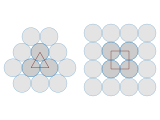
\includegraphics{img/parameter_study/packings}
    \caption{Particle Packings Regarded in this Investigation}
    \label{fig:parameter_study/packings}
\end{figure}

In a regular packing of equal circles each pore in the packing shows equal evolution due to symmetry.
Three different packings, displayed in \autoref{fig:parameter_study/packings}, shall be investigated here, which resemble common configurations of sphere packings:
\begin{description}
    \item[Triangle] the densest possible packing of circles with particles at the corners of an equal sided triangle, resembles a $\\left{ 111 \right}$ cut through a face-centered cubic cell
    \item[Square] the loosest regular packing with particles at the corners of a square, resembles a $\\left{ 100 \right}$ cut through a simple cubic cell
    \item[Rhombus] an intermediate packing with particles at the corners of a rhombus of \angle{70}, resembles a $\left{ 110 \right}$ cut through a body centered cubic cell
\end{description}
The main difference between these packings is the size and the shape of the pore formed by them.
As a reference the usual two-particle model (pair case) is taken alongside.

These packings are expected to show only effects of pore closing, but otherwise behave in a fully symmetric way equivalently to the pair case, as all particles are of equal size, shape and material properties.
So in a second step, one of the particles will be given a surface diffusion coefficient 100 times smaller than the other ones to regard hindering of sintering by the presence of an inert particle.
This particle is shown with brown stroke in \autoref{fig:parameter_study/packings}.

\subsection{Discussion of the Results}

\begin{figure}
    \includegraphics{sim/packings/shrinkage}
    \caption{Comparison of Shrinkages Obtained for the Investigated Packings}
    \label{fig:packings/shrinkage}
\end{figure}

\autoref{fig:packings/shrinkage} shows the shrinkage for the distinct packings obtained from the simulations.
The shrinkage is calculated in all cases using the distance approach and the polygon approach as discussed in \autoref{sec:packings}, except for the pair for which the polygon approach is not applicable.
Note, that the distinct cases all show the equal behavior in early stages.
At some point, specific for the respective case, the curve deviates rapidly to higher shrinkages from the reference two-particle model.
This point is related to the pore closing and the change of its shape characteristic from concave to convex, as is discussed in \textcite{Tikare2003}.
Therefore, the deviation occurs earlier for the more dense packed cases, in order: triangle, rhombus, square.

At the point where the pore was completely closed, the simulations were cancelled, as the current model does not support triple points yet.
Complete closure was determined at the point, were the last surface node between two neck nodes was removed by the neck remeshing procedure.
As the model is only aimed at initial and intermediate sintering stages, this problem can be neglected.

Note also, that the methods of calculating the shrinkage are not equivalent to each other.

\begin{figure}
    \begin{subfigure}{0.5\linewidth}
        \includegraphics{img/packings/pair/evolution}
        \caption{Pair}
        \label{fig:packings/pair/evolution}
    \end{subfigure}%
    \begin{subfigure}{0.5\linewidth}
        \includegraphics{img/packings/triangle/evolution}
        \caption{Triangle}
        \label{fig:packings/triangle/evolution}
    \end{subfigure}
    \begin{subfigure}{0.5\linewidth}
        \includegraphics{img/packings/square/evolution}
        \caption{Square}
        \label{fig:packings/square/evolution}
    \end{subfigure}%
    \begin{subfigure}{0.5\linewidth}
        \includegraphics{img/packings/rhombus/evolution}
        \caption{Rhombus}
        \label{fig:packings/rhombus/evolution}
    \end{subfigure}%
    \caption{Geometry Evolutions of the Distinct Cases}
    \label{fig:packings/evolution}
\end{figure}
